[8~r\textsuperscript{o}] sed in quam ista cadant 
%Zeitz auskommentiert\begin{wrapfigure}{l}{0.35\textwidth}                    
%                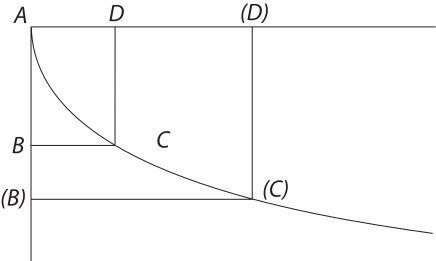
\includegraphics[width=0.34\textwidth]{images/35_5_8r1}\\\rule[0cm]{1.5cm}{0cm}\textit{[Fig. 8]}
%                        %\caption{Bildbeschreibung}
%                        \end{wrapfigure}
                        figuram subtilius inquirendum est,\rule[0cm]{0cm}{15pt} cum redeatur ad mirabilem illam methodum Tangentium inversam. Ego vero investigandum adhuc censeo an non alia 
                     supersit proclivior via. 
 Si \textit{AB} tempus \textit{y} 
\edtext{et \textit{BC} \textit{x} spatium illo tempore decursum}{\lemma{\textit{y}}\Afootnote{ \textit{ (1) }\ decursum \textit{ (2) }\ et [...] decursum \textit{ L}}}, 
utique erit \textit{AC(C)} parabolica, cujus vertex \textit{A} tangens verticis \textit{AB(B)}. Ergo si spatia sumantur uniformiter crescentia \textit{x}; [\textit{AB}]
\edtext{}{\Afootnote{\textit{AD}\textit{\ L \"{a}ndert Hrsg. } }}, erunt tempora ut applicatae parabolae;
 \edtext{et crementa}{\lemma{et}\Afootnote{ \textit{ (1) }\ quolibet  \textit{(a)}\ temporis momento \textit{(b)}\ spatii puncto erunt \textit{ (2) }\ crementa temporum \textit{ L}}} temporum 
\edtext{\textit{z}, 
                      }{\lemma{\textit{z},}\Afootnote{ \textit{ (1) }\ ut \textit{ (2) }\ seu \textit{ L}}} seu tempora quolibet spatii \edtext{[puncto]}{\lemma{momento}\Afootnote{\textit{\ L \"{a}ndert Hrsg.}}} percursa, erunt ut differentiae applicatarum parabolae, nempe:
 $\surd 2ax\sqcap y$ applicata parabolae, duarum applicatarum differentia: $\sqrt{2ax}-\sqrt{2ax-2a\beta,} \sqcap z$.                   
                      unde $\surd 2ax \sqcap z + \sqrt{2ax-2a\beta}$. et quadrando utrobique: $\ovalbox{2ax}\sqcap z^2+2z\sqrt{2ax-2a\beta}+ \ovalbox{2ax}-2a\beta$ sive: $-2z\sqrt{2ax-2a\beta}\sqcap z^2-2a\beta$, sive 
                      $4z^2 2ax - 4z^2 \ovalbox{2}a \beta \sqcap z^4 \ovalbox{$-4z^2a\beta$} +4a^2 \beta^2$
                     et ordinando 
                     \begin{edarrayl}
                     z^4\hspace{-8pt}&-8ax z^2 +4a^2 \beta^2 \sqcap 0\\
                     &+ 4a\beta ..
                     \end{edarrayl} quae aequatio ultra dividi non potest. 
Quod si reliquissemus: $\surd2ax-\sqrt{2ax-2a\beta}\sqcap z$, fiet: $2ax - 2\sqrt{4a^2 x^2 -4a^2 \beta x}+2ax-2a\beta\sqcap z^2$, sive: $4ax-2a\beta - z^2 \sqcap 2 \sqrt{4a^2 x^2 -4a^2 \beta x}$, et quadrando: $\ovalbox{$16a^2 x^2 -16a^2 \beta x$}-8axz^2 +4a^2 \beta^2 + 4a\beta z^2 + z^4 \sqcap \ovalbox{$16a^2 x^2 - 16a^2 \beta x$}$ sive $\displaystyle 8ax \sqcap \frac{z^2 + 2a\beta ,}{z}\raisebox{1mm}[0mm][0mm]{\boxed{}}$ itaque \edtext{si}{\lemma{itaque}\Afootnote{ \textit{ (1) }\ qualiacunque sint \textit{ (2) }\ si \textit{ L}}} crementa temporum in motu uniformiter accelerato\protect\index{Sachverzeichnis}{motus!uniformiter acceleratus} sint \textit{z} erunt spatia in quibus \edtext{decursis illa contingunt}{\lemma{quibus}\Afootnote{ \textit{ (1) }\ illa contingunt \textit{ (2) }\ decursis illa contingunt \textit{ L}}} $z^2 + 2a\beta , \smallsmile 8az$. Contra: ut investigetur valor ipsius \textit{z}, fiet:\newline
                 %    $\displaystyle z^4- 8ax\hspace{3pt}z^2+4a\beta ..\left\{\begin{array}{ll}\displaystyle+64a^2x^2&\sqcap\\\displaystyle-64a^2\beta x&\\\displaystyle \frac{+16a^2\beta^2}{4}&\end{array}\right.$
                           %    $\displaystyle z^4- 8ax\hspace{3pt}z^2+4a\beta ..\Bigg\{\begin{array}{ll}\displaystyle+64a^2x^2&\sqcap\\\displaystyle-64a^2\beta x&\\\displaystyle \frac{+16a^2\beta^2}{4}&\end{array}
                               $\begin{array}{r}\displaystyle z^4- 8ax\hspace{3pt}z^2\\+4a\beta ..\\\rule[0cm]{0cm}{20pt}
                               \end{array}
                               \Bigg\{\begin{array}{ll}\displaystyle+64a^2x^2&\sqcap\\\displaystyle-64a^2\beta x&\\\displaystyle \frac{+16a^2\beta^2}{4}&\end{array}
                     \begin{array}{ll}\displaystyle+8a^2x^2&\text{, adeoque }z^2 - 4ax +2a\beta\\\displaystyle-8a^2\beta x&\\\displaystyle \ovalbox{$+4a^2\beta^2\hspace{-35pt}\raisebox{-13pt}{$-4a^2\beta^2$}$}&\end{array}$\newline
                      $  \sqcap$ $2a \sqrt{2x^2 - 2\beta x}$ sive $z^2$ $\sqcap$ $4ax - 2a\beta + 2a \sqrt{2x^2 - 2\beta x}$ \edtext{}{\lemma{$2a\sqrt{2x^2 - 2\beta x}$}\Bfootnote{Der korrekte Faktor vor der Wurzel lautet \textit{4a}. Der Fehler wirkt sich in der Rechnung bis zur Bestimmung des Ausdrucks f\"ur x S. 535 Z. 11 aus, wo wir auch das richtige Ergebnis angeben.}} sive $z$ $\sqcap$ $\sqrt{4ax - 2a\beta + 2a\sqrt{2x^2 - 2\beta x}}$. Quodsi \edtext{ergo cum temporum seu virium crementa}{\lemma{ergo}\Afootnote{ \textit{ (1) }\ motus est uniformiter acceleratus\protect\index{Sachverzeichnis}{motus!uniformiter acceleratus|textit} \textit{ (2) }\ cum motus est uniformiter acceleratus\protect\index{Sachverzeichnis}{motus!uniformiter acceleratus|textit}, spatia \textit{ (3) }\ cum temporum seu virium crementa \textit{ L}}}, \textit{z} sunt in spatiorum percursorum\protect\index{Sachverzeichnis}{spatium!percursum} \edtext{\textit{x}}{\lemma{percursorum}\Afootnote{ \textit{ (1) }\ \textit{z} \textit{ (2) }\ \textit{x} \textit{ L}}}, ratione quae exprimitur; motus\protect\index{Sachverzeichnis}{motus!uniformiter acceleratus} \edtext{est quolibet temporis momento uniformiter acceleratus}{\lemma{est}\Afootnote{ \textit{ (1) }\ uniformiter \textit{ (2) }\ quolibet temporis momento uniformiter acceleratus \textit{ L}}}, quaeritur cum \edtext{crementa virium}{\lemma{cum}\Afootnote{ \textit{ (1) }\ in spa \textit{ (2) }\ crementa virium \textit{ L}}} \textit{z} sunt in spatiorum percursorum\protect\index{Sachverzeichnis}{spatium!percursum} \edtext{\textit{n}}{\lemma{percursorum}\Afootnote{ \textit{ (1) }\ \textit{z} \textit{ (2) }\ \textit{n} \textit{ L}}} ratione reciproca, seu cum $\displaystyle z \sqcap \frac{a^2}{n}\rule[-4mm]{0mm}{10mm}$. quae tum \edtext{futura sit}{\lemma{tum}\Afootnote{ \textit{ (1) }\ fuerit \textit{ (2) }\ futura sit \textit{ L}}} ratio accelerationis\protect\index{Sachverzeichnis}{acceleratio}, in quolibet temporis momento. Nimirum ut aequatio $z \sqcap \sqrt{4ax - 2a\beta + 2a\sqrt{2x^2 - 2\beta x}}$ sit ad hyperbolam secundum asymptotos, sive aequivaleat huic: $\displaystyle \frac{a^2}{n}$, fiet aequatio inter haec duo: %\pend \pstart 
                     $\displaystyle \sqrt{4ax - 2a\beta + 2a \sqrt{2x^2 - 2\beta x}}\sqcap \frac{a^2}{n}$. cujus aequationis ope quaeratur valor ipsius \textit{x}. \edtext{nempe}{\lemma{\textit{x}.}\Afootnote{ \textit{ (1) }\ et repertus \textit{ (2) }\ nempe \textit{ L}\protect\rule[0cm]{1.5cm}{0cm}}} $4ax - 2a\beta + 2a \sqrt{2x^2 - 2\beta x}\sqcap \displaystyle\frac{a^4}{n^2}$. sive %\pend \pstart 
                     $\displaystyle 2a\sqrt{2x^2 - 2\beta x}\sqcap \displaystyle\frac{a^4}{n^2} - 4ax + 2a\beta$, et quadrando: \rule[0cm]{0pt}{20pt}%\pend \pstart 
                     $\displaystyle \ovalbox{$8a^2x^2$} \hspace{-26pt}\raisebox{-3pt}{,,} \hspace{23pt}\ovalbox{$-8a^2\beta x$} \hspace{-26pt}\raisebox{-5pt}{,} \hspace{23pt}\sqcap \frac{a^8}{n^4}-\frac{8a^5}{n^2}x+4\frac{a^5\beta,}{n^2}+\ovalbox{16} \hspace{-14pt}\raisebox{-3pt}{,,} \hspace{11pt}\hspace{-14pt}\raisebox{-13pt}{8} \hspace{11pt}a^2x^2-\ovalbox{16} \hspace{-11pt}\raisebox{-3pt}{,} \hspace{11pt}\hspace{-14pt}\raisebox{-13pt}{8} \hspace{11pt}a^2\beta x +4a^2\beta^2$ et ordinando: \\
                     $\begin{array}{rll}
                 %   \displaystyle  x^2-\beta \rule[0pt]{8pt}{0pt}&x&+ \displaystyle\frac{a^6}{8n^4}\hspace{3pt}\sqcap 0\rule[-0.5cm]{0cm}{1cm}\\
                  %\displaystyle   -\frac{8a^3}{n^2}&\raisebox{2pt}{.}&\displaystyle+\frac{4a^3 \beta}{8n^2}\rule[-0.5cm]{0cm}{1cm}\\
                   \displaystyle  x^2-\hspace{6pt}\beta \hspace{4pt}x&+ \displaystyle\frac{a^6}{8n^4}\hspace{3pt}\sqcap 0\rule[-0.5cm]{0cm}{1cm}\\
                  \displaystyle   -\frac{8a^3}{n^2}\hspace{4pt}\raisebox{2pt}{.}&\displaystyle+\frac{4a^3 \beta}{8n^2}\rule[-0.5cm]{0cm}{1cm}\\
                   \displaystyle   &\displaystyle+ \frac{4\beta ^2}{8}.&
                     \end{array}$\\
                     %Alternativanfang
                 %    $\displaystyle x^2\hspace{4pt}-\beta\hspace{4pt}x + \frac{a^6}{8n^4}\hspace{3pt}\sqcap 0\\\displaystyle \rule{0cm}{0.7cm}\rule{81pt}{0pt}-\frac{8a^3}{n^2}\raisebox{2pt}{.}+\frac{4a^3 \beta}{8n^2}\\ \rule{0cm}{0.7cm}\rule{114pt}{0pt} + \frac{4\beta ^2}{8}$. \\
                     %Alternativende
                %     sive $\displaystyle x^2-\beta x -\frac{8a^3}{n^2}\cdotp\left\{\begin{array}{ll}\displaystyle+\beta^2&\sqcap\\\displaystyle+\frac{16a^3\beta}{n^2}&\\\displaystyle\frac{\displaystyle+\frac{64a^6}{n^4}}{4}&\end{array}\right.\left\{\begin{array}{ll}\displaystyle\beta^2&\displaystyle-\frac{a^6}{8n^4}\\\displaystyle\frac{16a^3\beta}{n^2}&\displaystyle-\frac{a^3\beta}{2n^2}\\\displaystyle\frac{\displaystyle+\frac{64a^6}{n^4}}{4}&-2\beta^2\end{array}\right.$ \\ 
                        sive  \protect \raisebox{10pt}{$\begin{array}{r}
                     \displaystyle x^2-\hspace{8pt}\beta \rule[-14pt]{0pt}{33pt}\hspace{4pt}x\\
                     \rule[0pt]{10pt}{0pt}   -\displaystyle\frac{8a^3}{n^2}\hspace{4pt}\cdotp\\
                        
                        \end{array}$}
                      $  \left\{\begin{array}{ll}\displaystyle+\beta^2&\rule[-12.5pt]{0pt}{29.5pt}\\\vspace{0.2cm}\displaystyle+\frac{16a^3\beta}{n^2}&\sqcap\\\underline{\displaystyle+\frac{64a^6}{n^4}}&\end{array}\right.\left\{\begin{array}{ll}\displaystyle\beta^2&\displaystyle-\frac{a^6}{8n^4}\vspace{0.2cm}\\\displaystyle\frac{16a^3\beta}{n^2}&\displaystyle-\frac{a^3\beta}{2n^2}\vspace{0.2cm}\\\underline{\displaystyle+\frac{64a^6}{n^4}}&-2\beta^2\end{array}\right.$
                       \\ \rule[0cm]{4cm}{0cm}4\hspace{2.5cm}4\\
                  \rule[-12pt]{0pt}{38pt}   sive
                     \def\leibdashvv{\diatop[$\vspace{10pt}-$|$|$]}
                     \def\leibdashv{\diatop[$\leibdashvv$|$\hspace{-5.15pt}\dashv$]}
                    \def\leibvdash{\protect\raisebox{10.5pt}{\protect\scalebox{1}[-1]{$\leibdashv$}}}                 
                      [ $\displaystyle \leibdashv x \leibvdash \frac{\beta^2}{2} \sqcap\sqrt{- \frac{\beta^2}{4}+\frac{a^6}{8n^4}} \\\rule{60pt}{0pt}\frac{a^3}{2n^2}$]\edtext{}
                   %   {\Afootnote{ $\displaystyle {\diatop[${\diatop[$\vspace{10pt}-$|$|$]}$|$\hspace{-5.15pt}\dashv$]} \hspace{2pt}x \hspace{5pt} {\protect\raisebox{10.5pt}{\protect\scalebox{1}[-1]{${\diatop[${\diatop[$\vspace{10pt}-$|$|$]}$|$$}} \hspace{-5.15pt}\dashv$]}  \hspace{5pt} \protect\frac{\beta^2}{2} \protect\sqcap \protect\sqrt{ \protect\llcorner \protect\frac{1}{4} - 2 \protect\lrcorner \beta^2,, + \protect\llcorner 4 - \protect\frac{1}{2}a \protect\lrcorner \protect\frac{a^3\beta}{n^2},, + \protect\llcorner8 - \protect\frac{1}{8}\protect\lrcorner \protect\frac{a^6}{n^4}} \protect\frac{4a^3}{n^2}$ \textit{\ L \"{a}ndert Hrsg. } }}.
                   %   {\Afootnote{$\displaystyle \leibdashv \hspace{5pt} x \hspace{5pt} \leibvdash \hspace{5pt} \protect\frac{\beta^2}{2} \protect\sqcap \protect\sqrt{ \protect\llcorner \protect\frac{1}{4} - 2 \protect\lrcorner \beta^2,, + \protect\llcorner 4 - \protect\frac{1}{2}a \protect\lrcorner \protect\frac{a^3\beta}{n^2},, + \protect\llcorner8 - \protect\frac{1}{8}\protect\lrcorner \protect\frac{a^6}{n^4}} \protect\frac{4a^3}{n^2}$ \textit{\ L \"{a}ndert Hrsg. } }}.
                         {\Afootnote{$\protect\begin{array}{rl}\displaystyle \leibdashv \hspace{5pt} x \hspace{5pt} \leibvdash \hspace{5pt} \displaystyle\protect\frac{\beta^2}{2} &\protect\sqcap\hspace{5pt} \protect\sqrt{ \protect\llcorner \displaystyle\protect\frac{1}{4} - 2 \protect\lrcorner \beta^2,, + \protect\llcorner 4 - \displaystyle\protect\frac{1}{2}a \protect\lrcorner \displaystyle\protect\frac{a^3\beta}{n^2},, + \protect\llcorner8 - \displaystyle\protect\frac{1}{8}\protect\lrcorner \protect\frac{a^6}{n^4}}\vspace{0.1cm}\\ \displaystyle\protect\frac{4a^3}{n^2}&\protect\end{array}$ \textit{\ L \"{a}ndert Hrsg. } }}.
                         \pend
                         \pstart
                       Habetur ergo valor ipsius \textit{x} qui insertus in aequatione $\surd 2ax\hspace{5pt} \sqcap\hspace{5pt} y$. exprimit relationem spatiorum et temporum. Imo festinandum lente, hic enim alioquin horribilem paralogismum committeremus. Sane verum est, summam omnium \textit{z} haberi posito earum valore expresso per \textit{x} sed non datur in his regressus; et non ideo habetur qualis futura sit \textit{y}.\pend \pstart Quaestio enim huc proprie redit: data est aequatio: $\surd 2ax \sqcap y$. Quaeritur, quomodo \edtext{explicanda}{\lemma{quomodo}\Afootnote{ \textit{ (1) }\ investiganda \textit{ (2) }\ exprimenda \textit{ (3) }\ explicanda \textit{ L}}} sit quantitas \textit{x}, per aliquam quandam incognitam ut \textit{n}, ut scilicet differentia duarum \textit{y} relinquat $\displaystyle \frac{a\beta}{n}$. Hoc autem problema \edtext{calculo}{\lemma{}\Afootnote{calculo \textit{ erg.} \textit{ L}}} solvi non potest, nisi ex data Hyperbolae quadratura, lineis autem solvi potest \edtext{per quadraturam Hyperbolae Geometricam}{\lemma{potest}\Afootnote{ \textit{ (1) }\ ope quadraturae Hyperbolae Geometricae \textit{ (2) }\ per quadraturam Hyperbolae Geometricam \textit{ L}}}, quae a me inventa est. Notabilis ista inquisitio est, ita enim duae methodi diversissimae circa idem problema \edtext{[habentur]}{\lemma{habuntur}\Afootnote{\textit{\ L \"{a}ndert Hrsg. } }}, et ratio exhibetur distortam illam et in se reflexam methodum tangentium inversam, revocandi ad simplicem et ad quadraturas.
                       \pend
                        % \vspace*{8mm}
                        \clearpage
                          \pstart
    \centering        \lbrack\textit{Teil 2}\rbrack
            \pend
                       \pstart
                      [9 r\textsuperscript{o}] Decembris 1674 
                       \pend
                       \pstart
                       \centering
                       \textso{Calculus Elasticus}.\footnote{\textso{Calculus Elasticus} \textit{doppelt unterstrichen}}\pend
%  Zeitz auskommentiert                     \begin{center}                    
%                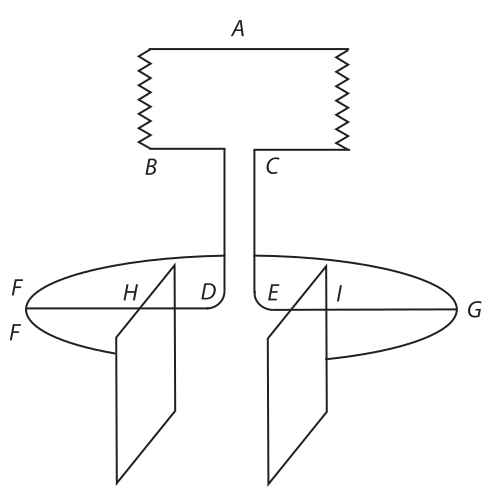
\includegraphics[width=0.5\textwidth]{images/35_5_9r1}\\%\rule[0cm]{1.5cm}{0cm}
%                \textit{[Fig. 1]}
%                        %\caption{Bildbeschreibung}
%                        \end{center}
                        \pstart
              Sit follis \textit{AB} cujus asser mobilis \textit{A} immobilis \textit{B} in quo fixus canalis \edtext{\textit{CDE} desinens}{\lemma{\textit{CDE}}\Afootnote{\textit{ (1) } extendens \textit{ (2) } desinens \textit{L}}} se sub finem in \textit{DE}, in Tabulam \textit{FG} in cujus diametro mobiles asseres duo dum follis deprimitur flatu aeris aut aquae asseres a se invicem distendent. Ajo si distantiae asserum sint ut \edtext{numeri,}{\lemma{numeri,}\Afootnote{\textit{ (1) } tempora quibus in \textit{ (a) } eam distantiam \textit{ (b) } eas distantias ferantur \textit{ (2) } vires quas in iis distantiis acquisierint  \textit{L}}}  vires quas in iis distantiis acquisierint fore ut \edtext{logarithmos}{\lemma{logarithmos}\Afootnote{\textit{ (1) } modo asseres ponantur non ultra ire, quam cogit follis \textit{ (2) } modo aequabili semper motu claudatur follis \textit{L}}} modo aequabili semper motu claudatur follis. Hinc vicissim \edtext{si tempora sint ut numeri, seu exponentes, aperturae erunt}{\lemma{si}\Afootnote{\textit{ (1) }  apertura \textit{ (2) } tempora [...] erunt \textit{L}}}  ut cujusdam numeri secundum eum exponentem potestates. Ratio hujus rei est, quod vires flatus impellentis, sunt in spatiorum ratione \edtext{reciproca.}{\lemma{reciproca.}\Afootnote{\textit{ (1) } In quolibet ergo spatio in \textit{ (2) } Motus ergo acceleratio est  \textit{L}}}  Motus ergo acceleratio\protect\index{Sachverzeichnis}{acceleratio} \edtext{est in spatiis quibuslibet per}{\lemma{est}\Afootnote{\textit{ (1) } per \textit{ (2) }  in spatiis quibuslibet \textit{L}}} \edtext{crementa virium}{\lemma{per}\Afootnote{\textit{ (1) } incrementa \textit{ (2) } crementa virium \textit{L}}} spatiis reciproca, seu proportionalia applicatis \edtext{hyperbolae. Ergo summae virium ut }{\lemma{hyperbolae}\Afootnote{\textit{ (1) }, ergo temporum decrementa. Jam virium incrementa sunt in \textit{ (2) } . Ergo summae virium ut Logarithmi \textit{L}}}\edtext{Logarithmi. Temporum autem crementa virium crementis reciproce proportionalia.}{\lemma{Logarithmi.}\Afootnote{\textit{ (1) } Sed ut verum dicam, \textit{ (2) }Temporum [...] proportionalia. \textit{L}}} Ergo spatiis directe. Ergo summae temporum quibus spatia percurruntur erunt ut spatiorum quadrata. Idemque est si embolum \textit{EFG} ex spatio extrudi putes, elaterio aeris compressi ponendo vim expellendi esse in reciproca spatiorum ratione. Sed jam re rectius perspecta hoc verum esse non video: foret \edtext{si}{\lemma{si}\Afootnote{\textit{ (1) } libertas \textit{ (2) } poneret \textit{L}}} \edtext{poneret vas ita compressum, in vacuo}{\lemma{poneret}\Afootnote{\textit{ (1) }aer in vacuo, \textit{ (2) }vas ita compressum, in vacuo, \textit{L}}}, ita ut aer summam habeat se restituendi libertatem. Et idem de folle, si is ponatur \edtext{infinite largus,}{\lemma{infinite}\Afootnote{\textit{ (1) } magnus \textit{ (2) } largus \textit{L}}} \edtext{seu}{\lemma{largus,}\Afootnote{\textit{ (1) } seu \textit{ (2) }  nam \textit{ (3) } seu \textit{L}}} si flumen in angustias compellendum sit infinite magnum. Hic vero sciendum est terminum esse virium, tunc cum aequalitas facta est inter aerem internum et externum, sive \edtext{cum Aer folles egrediens inter angustias}{\lemma{cum}\Afootnote{\textit{ (1) } asser a \textit{ (2) } Aer follis \textit{ (3) } Aer folles egrediens inter angustias \textit{L}}} et asser comprimens in folle eadem celeritate ferri possunt. Itaque cum absolute loquendo verum sit vires esse in spatiorum ratione reciproca, vires tamen hic aestimandae a viribus duorum spatiorum externi et interni virium differentiis; sive a differentiis materiarum eorundem spatiorum. Aliter embolus \textit{FG} in canalem \textit{AD} intrusus interstitia \textit{HI} si potest reddet ampliora, donec fiat $HI \sqcap FG$.
              \pend
% Zeitz auskommentiert             \begin{center}                    
%                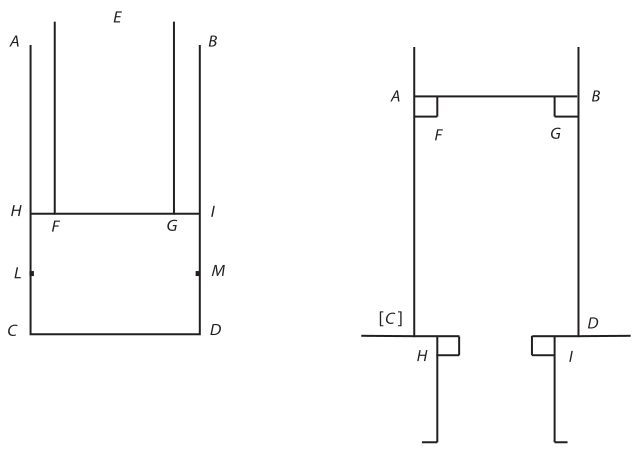
\includegraphics[width=0.8\textwidth]{images/35_5_9r2}\\%\rule[0cm]{1.5cm}{0cm}
%                \textit{[Fig. 2]}\rule[0cm]{5cm}{0cm}\textit{[Fig. 3]}\rule[0cm]{0.5cm}{0cm}
%                        %\caption{Bildbeschreibung}
%                        \end{center}
              \pstart
              Eodem ergo modo in Elateriis imaginabimur poros reddi angustos, ut materia per eos mota difficultatem transeundi experiatur ne proinde moveatur solito celerius. Itaque aestimanda materiae sive potius spatii quantitas, et ducenda in differentiam celeritatum. Durante autem motu crescit spatium celeritas decres\-cit. Spatia per se patent; celeritas autem aestimanda est a materiae transeuntis \edtext{quantitate, vel etiam a}{\lemma{quantitate,}\Afootnote{\textit{ (1) } sed de his suo loco a\textit{ (2) } vel etiam a \textit{L}}} quantitate detorsionis corporis transire conantis a motu suo.
              \pend
              \pstart
              Caeterum illud manifestum est, demonstrationes \edtext{Hugenianas}{\lemma{Hugenianas}\Afootnote{\textit{ (1) } circa Cycloeidem \textit{ (2) } de Cycloeidis \textit{L}}} \edtext{de Cycloeidis isochronismo}{\lemma{Cycloeidis}\Afootnote{\textit{ (1) } de isochronismis \textit{ (2) } isochronismo \textit{L}}}\edtext{}{\lemma{isochronismo}\Bfootnote{\textsc{Chr. Huygens}, \cite{00123}\textit{Horologium oscillatorium}, Paris 1673, S.~57f. (\textit{HO} XVIII, S.~185\textendash187).}} nihil ad rem pertinere; quia pendent ex rigorosa observatione regularum Galilaei de acceleratione gravium; at ea acceleratio\protect\index{Sachverzeichnis}{acceleratio}: at eas regulas a natura non observari ex \edtext{eo patet,}{\lemma{eo}\Afootnote{\textit{ (1) } pendet \textit{ (2) } patet \textit{L}}} \edtext{quod pendula}{\lemma{quod}\Afootnote{\textit{ (1) } corpora \textit{ (2) } pendula \textit{L}}} non tam alte ascendunt quam decidere. Eadem ergo causa quae pendulorum ascensum impedit et temporum spatiorumque rationem, adeoque et isochronismum si quis demonstrari posset. Cumque differentia sit valde sensibilis, hinc sequitur eam demum isochronismi demonstrationem ad rem pertinere, quae simul et rationem decrescentium vibrationum reddat.